\documentclass[conference]{IEEEtran}

\usepackage[utf8]{inputenc}
\usepackage[spanish]{babel}
\usepackage{cite}
\usepackage{amsmath,amssymb,amsfonts}
\usepackage{algorithmic}
\usepackage{graphicx}
\usepackage{textcomp}
\usepackage{booktabs}
\usepackage{tabularx}
\usepackage{subcaption}
\newcolumntype{C}{>{\centering\arraybackslash}X}    % centered flexible tabularX column
\renewcommand{\spanishtablename}{Tabla}
\usepackage[
    group-digits=integer,
    group-minimum-digits=4,
    input-decimal-markers={.},
    output-decimal-marker={,}]{siunitx}
\def\BibTeX{
    {\rm B\kern-.05em{\sc i\kern-.025em b}\kern-.08em
    T\kern-.1667em\lower.7ex\hbox{E}\kern-.125emX}
}

\usepackage{url}
\renewcommand{\UrlFont}{\ttfamily\small}
\urldef{\TheRepoUrl}\path{https://github.com/nico-ralf-ii-fpuna/tfg}

% Definicion de glosarios para simbolos y acronimos
\usepackage{datatool}
\usepackage[nomain,nonumberlist,toc]{glossaries}
\setglossarystyle{altlong4col}
\newglossary[sim1]{sim2}{sim3}{sim4}{Lista de Símbolos}
\newglossary[acr1]{acr2}{acr3}{acr4}{Lista de Acrónimos}
\makeglossaries
%
% Lista de símbolos
%

\newglossaryentry{sim3:g}{
    type=sim2,
    name=$G$,
    description={conjunto de grupos de peticiones HTTP agrupadas por
        método y URL}
}
\newglossaryentry{sim3:gi}{
    type=sim2,
    name=$G_{i}$,
    description={el grupo \textit{i} de peticiones HTTP con un mismo
        método y una misma URL}
}
\newglossaryentry{sim3:qi}{
    type=sim2,
    name=$Q_{i}$,
    description={lista de parámetros del \textit{query string} de las
        peticiones HTTP del grupo $G_{i}$}
}
\newglossaryentry{sim3:bi}{
    type=sim2,
    name=$B_{i}$,
    description={lista de parámetros del cuerpo de las peticiones HTTP
        del grupo $G_{i}$}
}
\newglossaryentry{sim3:fi}{
    type=sim2,
    name=$F_{i}$,
    description={conjunto de vectores de \textit{features} que representan
        las peticiones HTTP del grupo $G_{i}$}
}
\newglossaryentry{sim3:fij}{
    type=sim2,
    name=$\vec{f_{ij}}$,
    description={vector de \textit{features} que representa una petición
        HTTP del grupo $G_{i}$}
}
\newglossaryentry{sim3:ni}{
    type=sim2,
    name=$n_{i}$,
    description={cantidad de componentes de los vectores $\vec{f_{i}_{j}}$
        del conjunto $F_{i}$}
}
\newglossaryentry{sim3:m}{
    type=sim2,
    name=$m$,
    description={cantidad de \textit{features} extraídos por cada valor
        analizado}
}
\newglossaryentry{sim3:mi}{
    type=sim2,
    name=$M_{i}$,
    description={matriz de \textit{features} que representa las peticiones
        HTTP del grupo $G_{i}$ utilizadas para entrenamiento}
}
\newglossaryentry{sim3:wi}{
    type=sim2,
    name=$\vec{w_{i}}$,
    description={vector perpendicular al hiperplano del One-Class SVM
        para el grupo $G_{i}$}
}
\newglossaryentry{sim3:rhoi}{
    type=sim2,
    name=$\rho_{i}$,
    description={distancia al origen del hiperplano del One-Class SVM
        para el grupo $G_{i}$}
}
\newglossaryentry{sim3:nui}{
    type=sim2,
    name=$\nu_{i}$,
    description={parámetro del One-Class SVM que regula la fracción de
        muestras situadas al mismo lado del hiperplano que el origen
        para el grupo $G_{i}$}
}
\newglossaryentry{sim3:slacki}{
    type=sim2,
    name=$\xi_{i}$,
    description={lista de valores de holgura para el One-Class SVM del
        grupo $G_{i}$}
}
\newglossaryentry{sim3:gammai}{
    type=sim2,
    name=$\gamma_{i}$,
    description={parámetro del \textit{kernel} RBF que regula la
        dimensión de la región de influencia de cada muestra de
        entrenamiento para el grupo $G_{i}$}
}

%
% Lista de acrónimos
%

\newglossaryentry{acr3:name}{
    type=acr2,
    name={OCS-WAF},
    description={\textit{One-Class} SVM \textit{Web Application Firewall}}
}
\newglossaryentry{acr3:ids}{
    type=acr2,
    name=IDS,
    description=\textit{Intrusion Detection System}
}
\newglossaryentry{acr3:ips}{
    type=acr2,
    name=IPS,
    description=\textit{Intrusion Prevention System}
}
\newglossaryentry{acr3:hids}{
    type=acr2,
    name=HIDS,
    description=\textit{Host-based Intrusion Detection System}
}
\newglossaryentry{acr3:nids}{
    type=acr2,
    name=NIDS,
    description=\textit{Network-based Intrusion Detection System}
}
\newglossaryentry{acr3:http}{
    type=acr2,
    name=HTTP,
    description=\textit{Hypertext Transfer Protocol}
}
\newglossaryentry{acr3:ip}{
    type=acr2,
    name=IP,
    description=\textit{Internet Protocol}
}
\newglossaryentry{acr3:waf}{
    type=acr2,
    name=WAF,
    description=\textit{Web Application Firewall}
}
\newglossaryentry{acr3:ml}{
    type=acr2,
    name=ML,
    description=\textit{Machine Learning}
}
\newglossaryentry{acr3:occ}{
    type=acr2,
    name=OCC,
    description=\textit{One-Class Classification}
}
\newglossaryentry{acr3:svm}{
    type=acr2,
    name=SVM,
    description=\textit{Support Vector Machine}
}
\newglossaryentry{acr3:ocsvm}{
    type=acr2,
    name={One-Class SVM},
    description=\textit{One-Class Support Vector Machine}
}
\newglossaryentry{acr3:csic}{
    type=acr2,
    name=CSIC,
    description={Consejo Superior de Investigaciones Científicas de España}
}
\newglossaryentry{acr3:url}{
    type=acr2,
    name=URL,
    description=\textit{Universal Resource Locator}
}
\newglossaryentry{acr3:ascii}{
    type=acr2,
    name=ASCII,
    description=\textit{American Standard Code for Information Interchange}
}
\newglossaryentry{acr3:ghz}{
    type=acr2,
    name=GHz,
    description=\textit{Gigahertz}
}
\newglossaryentry{acr3:mb}{
    type=acr2,
    name=MB,
    description=\textit{Megabytes}
}
\newglossaryentry{acr3:gb}{
    type=acr2,
    name=GB,
    description=\textit{Gigabytes}
}
\newglossaryentry{acr3:ram}{
    type=acr2,
    name=RAM,
    description=\textit{Random Access Memory}
}
\newglossaryentry{acr3:rbf}{
    type=acr2,
    name=RBF,
    description=\textit{Radial Basis Function kernel}
}
\newglossaryentry{acr3:tpr}{
    type=acr2,
    name=TPR,
    description=\textit{True Positives Rate}
}
\newglossaryentry{acr3:fpr}{
    type=acr2,
    name=FPR,
    description=\textit{False Positives Rate}
}



\begin{document}
    \title{
        \gls{acr3:name}:
        un Web Application Firewall basado en anomalías
        con clasificadores \gls{acr3:ocsvm}
    }

    \author{
        \IEEEauthorblockN{Nico Epp}
        \IEEEauthorblockA{
            \textit{Facultad Politécnica}\\
            \textit{Universidad Nacional de Asunción}\\
            San Lorenzo, Paraguay\\
            nicoeppfriesen@gmail.com
        }
        \and
        \IEEEauthorblockN{Ralf Funk}
        \IEEEauthorblockA{
            \textit{Facultad Politécnica}\\
            \textit{Universidad Nacional de Asunción}\\
            San Lorenzo, Paraguay\\
            ralffunk0@gmail.com
        }
    }

    \maketitle

    \begin{abstract}
        Las vulnerabilidades en aplicaciones web presentan un gran riesgo, ya
        que estas pueden ser explotadas por atacantes maliciosos a través
        de Internet. Los \textit{Web Application Firewalls} (\gls{acr3:waf})
        pueden ser colocados frente a estas aplicaciones para detectar
        posibles ataques y de esta forma reducir estos riesgos.
        En este trabajo presentamos \gls{acr3:name}, un \gls{acr3:waf} que
        puede ser colocado frente a aplicaciones web para analizar los mensajes
        \gls{acr3:http} entrantes, con el fin de detectar mensajes anómalos
        que podrían contener ataques.
        Nuestra implementación, hecha en el lenguage de programación
        \textit{Python}, utiliza clasificadores \gls{acr3:ocsvm} para la
        detección, junto con procesos de extracción de características
        diseñados específicamente para mensajes \gls{acr3:http}.
        \gls{acr3:name} es entrenado con mensajes que representan el uso
        normal de las aplicaciones protegidas, y posteriormente, en la fase
        de detección, puede detectar mensajes anómalos o ataques.
        Usando esta estrategia de detección de anomalías, \gls{acr3:name}
        solamente necesita ser entrenado cuando haya cambios en las
        aplicaciones protegidas, por lo que la aparición de nuevos tipos de
        ataques no requiere volver a entrenarlo.
        Las pruebas realizadas para medir la eficacia de detección muestran
        que \gls{acr3:name} alcanza un \gls{acr3:tpr} promedio de \num{0.93},
        un \gls{acr3:fpr} promedio de \num{0.03} y un F$_{1}$-\textit{score}
        promedio de \num{0.95} para los conjuntos de datos públicos que
        utilizamos.
        Las pruebas también evidencian que las tareas de detección de \gls{acr3:name}
        no afectarían de forma notable el tiempo de respuesta de las aplicaciones
        protegidas. Además, puede ser entrenado con \num{100000} mensajes
        normales en unos pocos minutos.
        Finalmente, el código fuente de \gls{acr3:name} está disponible en
        un repositorio público bajo la dirección \TheRepoUrl, con la finalidad
        de que otros puedan reproducir nuestros resultados y extender este
        trabajo en futuras investigaciones.
    \end{abstract}

    \begin{IEEEkeywords}
        Sistemas de Detección de Intrusión (\gls{acr3:ids}),
        Web Application Firewall (\gls{acr3:waf}),
        ataques web,
        detección de anomalías,
        \gls{acr3:ocsvm}
    \end{IEEEkeywords}

    % the command '\include' adds pagebreaks, so we use '\input' instead
    \renewcommand{\thesection}{\arabic{section}}
\chapter{}
\label{chap:p_contenido}


\section{Motivación}

Las aplicaciones web han tenido un gran auge en la última década,
convirtiéndose en herramientas de uso masivo y frecuente para una
gran cantidad de usuarios. Pero debido a que las mismas son accesibles
a través de la red, están expuestas a una gran variedad de ataques
\cite{gimenez2015tfg}.
Muchas de las aplicaciones web actualmente no están construidas de acuerdo
a las mejores prácticas de seguridad, posibilitando que  dichas aplicaciones
queden vulnerables a diferentes ataques.
Esto se debe a la falta de consciencia sobre la importancia de la
seguridad y en muchos casos también a una falta de tiempo, ya que se
suele priorizar el desarrollo de funcionalidades por encima de la seguridad.
Esta es la situación de aplicaciones existentes como también lo
puede ser para aplicaciones futuras. Por lo tanto se necesitan soluciones
para mitigar los riesgos presentes.

En este trabajo nosotros investigaremos sobre mecanismos externos
especializados en la detección de ataques, con el fin de mitigar los
riesgos creados por las vulnerabilidades presentes en las aplicaciones web.
\bigskip

\gls{acr3:ids} son programas o dispositivos especializados para
monitorear las actividades en un sistema en busca de intrusiones no
autorizadas o posibles ataques \cite{scarfone2007guide}.
Las respuestas frente a posibles intrusiones pueden ser variadas, desde
envío de alertas hasta medidas concretas de mitigación y contención de
los posibles ataques. En este último caso se puede hablar también más
específicamente de \gls{acr3:ips} \cite{scarfone2007guide}.

Los \gls{acr3:ids} pueden basarse en varias fuentes de datos para sus
análisis, como por ejemplo el tráfico de una red o los registros de
acciones en un sistema operativo \cite{torranoGimenez2015study}.
Como las aplicaciones web utilizan mayormente el protocolo \gls{acr3:http}
\cite{fielding1999http} para sus comunicaciones, se necesita un
\gls{acr3:ids} que pueda monitorear el tráfico \gls{acr3:http},
analizando los paquetes enviados y recibidos a través de las conexiones
de red. En este caso se puede hablar más específicamente de \gls{acr3:waf}
\cite{torranoGimenez2015study}.

Nuestra propuesta puede ser considerada un \gls{acr3:waf} que tiene la
finalidad de detectar ataques contra aplicaciones web.
Cabe mencionar que debido a que \gls{acr3:waf} es un término más específico
que \gls{acr3:ids}, muchos de los conceptos expuestos a continuación aplican
a ambos términos, pero nosotros nos enfocamos únicamente en \gls{acr3:waf}
en este trabajo.
\bigskip

Los \gls{acr3:waf} pueden utilizar dos métodos distintos para la detección
de intrusiones.
Una forma puede ser la búsqueda de patrones de ataques conocidos, llamado
también método basado en firmas de ataques (\textit{signature-based
detection}).
Otro método empleado es la búsqueda de desviaciones o anomalías en el
tráfico \gls{acr3:http}, ya que estas pueden indicar ataques
(\textit{anomaly-based detection}) \cite{torranoGimenez2015study}.

Para que un \gls{acr3:waf} pueda utilizar eficazmente el método por firmas,
es necesario que el mismo mantenga una lista actualizada de las firmas de
todos los ataques conocidos. Esto resulta en un aumento del uso de tiempo y
recursos por parte de los \gls{acr3:waf} al momento de analizar el tráfico
de red, ya que la lista de ataques descubiertos crece y probablemente
nunca deje de crecer \cite{kruegel2003anomaly}.

El método de detección de anomalías no requiere una lista de firmas,
sino que en su fase de entrenamiento establece modelos que representan al
tráfico normal. Se basa en la premisa de que la mayoría de los ataques se
diferencian en alguna forma del tráfico normal.
En adelante usamos el término anomalía para referirnos a los ataques,
para ser consistentes con la literatura relacionada.
Así, durante la fase de monitoreo, este método compara el tráfico con los
modelos establecidos anteriormente con el fin de detectar desviaciones
significativas, es decir, aquellos paquetes \gls{acr3:http} que son
considerados anomalías \cite{kruegel2003anomaly}.
La fase de entrenamiento es obligatoria una vez al inicio del uso del
sistema y después solamente si hay cambios en el tráfico normal, por ejemplo
después de una actualización a una de las aplicaciones web que protege el
\gls{acr3:waf} en cuestión.

El método por anomalías tiene la ventaja de poder detectar anomalías
novedosas desde el momento que aparezcan, mientras que los métodos por
firmas dependen de la actualización de su lista de ataques conocidos
\cite{kruegel2003anomaly}.

A pesar de esto, \gls{acr3:waf} basados en anomalías no son tan comunes
como aquellos basados en firmas \cite{sommer2010outside}.
Esto se debe en parte a que suele ser más complicado establecer modelos
significativos para diferenciar muestras normales de anómalas y,
como consecuencia, hay menos posibilidades de detectar eficazmente
las anomalías. De esta manera los métodos por anomalías corren el peligro
de caer en extremos. Por un lado, si se concentran en detectar todas las
anomalías, pueden marcar equivocadamente muestras normales como anómalas
(más errores de falsos negativos). Por otro lado, si los métodos priorizan
no bloquear ninguna muestra normal, puede que muchas anomalías no sean
detectadas (más errores de falsos positivos) \cite{torranoGimenez2015study}.

Nuestra propuesta es un \gls{acr3:waf} basado en detección de anomalías
en el tráfico \gls{acr3:http}, buscando mejorar algunas de las propuestas
que ya han sido presentados por otros investigadores, como por ejemplo
Kruegel \cite{kruegel2003anomaly}, Giménez \cite{gimenez2015tfg} y
Torrano-Giménez \cite{torranoGimenez2015study}.
\bigskip

Para la detección de anomalías se puede utilizar varias estrategias.
Una opción es emplear herramientas estadísticas, como podemos ver en los
trabajos de Kruegel \cite{kruegel2003anomaly}, Giménez \cite{gimenez2015tfg}
y Torrano-Giménez \cite{torranoGimenez2015study}.
También se puede utilizar herramientas del área de \gls{acr3:ml}
\cite{torranoGimenez2015study} para tratar de detectar las anomalías.
Podemos ver ejemplos de estos en los trabajos de Sommer \cite{sommer2010outside},
Buczak \cite{buczak2016survey}, Parhizkar \cite{parhizkar2015oc}
y también en el trabajo ya mencionado de Torrano-Giménez
\cite{torranoGimenez2015study}.

Las herramientas de \gls{acr3:ml} han sido empleadas con mucho éxito
en varias áreas de la computación, como por ejemplo en sistemas de
recomendación de productos, clasificación de imágenes, reconocimiento
óptico de caracteres, entre otros \cite{torranoGimenez2015study}.

Una de las áreas de \gls{acr3:ml} son los problemas de clasificación, y la
detección de anomalías se puede encarar como un problema de esta área.
\gls{acr3:ml} puede utilizar varias herramientas para clasificar los
datos de entrada en varios grupos o clases.
En este contexto se habla de aprendizaje supervisado si se especifican
todas las clases posibles de antemano, usando solamente muestras para
el entrenamiento de las que se conocen sus clases. Muestras nuevas serán
asignadas a la clase a la que más se parezcan. Se habla de aprendizaje no
supervisado cuando no se provee muestras con clases conocidas de antemano
y la herramienta trata de encontrar las clases presentes en las muestras.
Este segundo caso está también estrechamente relacionado con los problemas
de agrupamiento (\textit{clustering}) \cite{torranoGimenez2015study}.

Aplicado a un \gls{acr3:waf}, se puede usar clasificación supervisada
con una clase para tráfico normal y otra (o también varias otras) para
tráfico anómalo.
Un primer desafío con este abordaje es que se necesita volver a entrenar
el clasificador cuando aparece un nuevo tipo de anomalía. Si no se
vuelve a entrenarlo con los nuevos tipos de anomalías, es posible que
el mismo clasifique equivocadamente una anomalía como normal en el caso
de una anomalía nueva que no se ajusta suficientemente a las clases de
anomalías vistas anteriormente por el clasificador.
Un segundo desafío es la necesidad de obtener muestras de todos los tipos
de anomalías conocidas para realizar un entrenamiento completo.

Estos dos desafíos se trata de superar con la estrategia conocida bajo el
nombre de \gls{acr3:occ} \cite{khan2009survey}. Se busca definir una sola
clase, la clase positiva, y clasificar las muestras de acuerdo a si
pertenecen o no a dicha clase. La fase de entrenamiento utiliza solamente
muestras de la clase positiva, de forma que una muestra que no se ajuste
a la clase positiva sea clasificada como no perteneciente a la misma
(clase negativa). Esto provee robustez frente a la aparición de muestras
negativas nuevas.
Esta estrategia ha sido utilizada con éxito en varias áreas, como detección
de spam, reconocimiento de rostros, detección de fallas en maquinarias, entre
otros \cite{khan2009survey}.
Aplicado a un \gls{acr3:waf}, la clase positiva estará conformada solamente
por el tráfico normal y todos los tipos de anomalías no pertenecerán a dicha
clase. Además, una gran ventaja con este abordaje es que no se necesita
muestras anómalas para el entrenamiento.

Para nuestra propuesta implementaremos un \gls{acr3:waf} que emplea
\gls{acr3:occ} con herramientas de \gls{acr3:ml} para detectar tráfico
\gls{acr3:http} anómalo. Con este abordaje solamente se necesita entrenar
una vez el clasificador con tráfico normal y, mientras no cambie la
aplicación, no debería ser necesario volver a entrenarlo, aún con
la aparición de nuevas anomalías.
\bigskip

Los algoritmos o herramientas utilizados en \gls{acr3:ml} son muy diversos,
como por ejemplo árboles de decisiones, redes neuronales, algoritmos
genéticos, entre otros \cite{torranoGimenez2015study}. Una de estas
herramientas, que ha sido utilizada con mucho éxito en las tareas de
clasificación, es la \gls{acr3:svm}. Una versión modificada del \gls{acr3:svm}
ha sido propuesta como una de varias alternativas para afrontar tareas de
\gls{acr3:occ} \cite{scholkopf2001estimating}.
Varios investigadores ya han empleado exitosamente este clasificador
\gls{acr3:ocsvm} en problemas de distintas áreas, como por ejemplo
clasificación de textos, clasificación de rostros, detección de spam,
detección de fallas en máquinas, entre otros \cite{khan2009survey}.

En este trabajo utilizaremos un \gls{acr3:ocsvm} para detectar tráfico
\gls{acr3:http} anómalo, combinando propuestas de varios investigadores
para obtener una alta eficacia del clasificador.
\bigskip

Para que un \gls{acr3:waf} basado en detección de anomalías pueda diferenciar
el tráfico \gls{acr3:http} normal del anómalo, es necesario que existan
características del tráfico que posibiliten esa diferenciación.
Ejemplos de esos rasgos pueden ser la longitud de la petición, la aparición
de ciertos caracteres con significado especial, entre otros
\cite{kruegel2003anomaly} \cite{nguyen2011application}.
Además se debe expresar esos rasgos en un formato procesable para las
herramientas de detección. La mayoría de las herramientas de \gls{acr3:ml}
no pueden trabajar con los datos crudos y necesitan un paso de
preprocesamiento de datos.
Asumiendo la existencia de esas características distintivas, el éxito
del \gls{acr3:waf} depende de encontrar dichos rasgos y de representarlos
en una forma entendible para el mecanismo de detección
\cite{torranoGimenez2015study}.
En esta parte el conocimiento experto sobre el tráfico \gls{acr3:http}
ayuda a seleccionar las características más útiles para ese fin.
Vemos un ejemplo de esta selección en los trabajos de Kruegel
\cite{kruegel2003anomaly} \cite{kruegel2005multi}, donde el autor utiliza
el conocimiento sobre la estructura de paquetes \gls{acr3:http} para obtener
rasgos más específicos, que denomina modelos de anomalías, y así mejorar la
detección.

En el área de \gls{acr3:ml}, las características de los datos de entrada se
representan con números, llamados también \textit{features}.
Por ejemplo para el caso de un \gls{acr3:waf}, el primer número puede
indicar la cantidad de caracteres de la petición \gls{acr3:http}, el
segundo la cantidad de dígitos presente y el tercero puede representar
la entropía calculada a partir de toda la petición.
De esta forma, la eficacia de detección de anomalías de nuestro clasificador
\gls{acr3:ocsvm} depende en gran parte de nuestros procesos de
\textit{feature extraction}, es decir, de los procesos de preprocesamiento
de datos que extraen las características distintivas del tráfico
\gls{acr3:http} y las representan con números \cite{torranoGimenez2015study}.

En este trabajo utilizaremos conocimiento experto sobre tráfico \gls{acr3:http}
para extraer características útiles para la detección de anomalías,
basandonos en los aportes de Kruegel y otros autores con trabajos relacionados.
Ya que trabajamos con un clasificador \gls{acr3:ocsvm}, en el resto del
trabajo utilizamos el término \textit{features} para referirnos a las
características mencionadas, para ser consistentes con la terminología
del área de \gls{acr3:ml}.


\section{Justificación}

Resumiendo lo expuesto anteriormente, en esta investigación combinamos
tres áreas de estudio para proponer una solución a la problemática
descrita. Dichas áreas se pueden observar también en la
\autoref{fig:areas_de_estudio}.

\begin{figure}[ht]
    \centering
    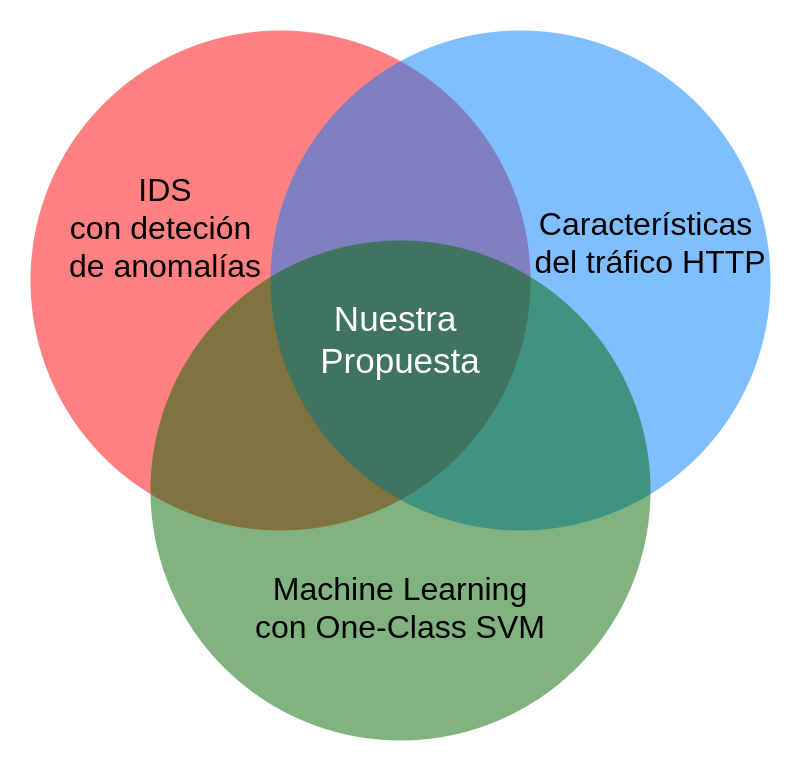
\includegraphics[width=0.6\linewidth]{images/venn-AreasDeEstudio.png}

    \caption{Diagrama de las áreas de estudio de la investigación}
    \label{fig:areas_de_estudio}
\end{figure}

\begin{itemize}
    \item
    \gls{acr3:ids} con en detección de anomalías:
    nuestra propuesta busca detectar posibles ataques al reconocerlos como
    tráfico anómalo.
    Utilizaremos el método de detección de anomalías debido a las ventajas
    mencionadas en la sección anterior.

    \item
    Caracteristicas del tráfico \gls{acr3:http}:
    utilizar conocimiento experto sobre la estructura del tráfico
    \gls{acr3:http} puede ayudar para diferenciar las peticiones normales
    de las anomalías o ataques, como se puede ver en los trabajos de Kruegel
    \cite{kruegel2003anomaly} \cite{kruegel2005multi}.

    \item
    \gls{acr3:ml} con \gls{acr3:ocsvm}:
    utilizamos este clasificador, debido a que otros investigadores obtuvieron
    buenos resultados al aplicarlo a distintos problemas de \gls{acr3:occ}
    \cite{khan2009survey} y la detección de tráfico anómalo se puede enfocar
    como un problema de \gls{acr3:occ}.
\end{itemize}

En los trabajos de Kruegel se combina las dos primeras áreas descritas
anteriormente, \gls{acr3:ids} y características del tráfico \gls{acr3:http}.
Sus ideas ya fueron aplicadas en varios trabajos en años subsecuentes,
pero no hemos encontrado una investigación que las combine con un
clasificador \gls{acr3:ocsvm}.

En nuestra opinión un \gls{acr3:waf} que combina las ideas de Kruegel
con este clasificador puede ser de gran utilidad para la protección de
aplicaciones web, y eso buscamos confirmar en el marco de este trabajo.


\section{Objetivos}

\subsection{Objetivo general}

Detectar tráfico \gls{acr3:http} anómalo entre aplicaciones web
y sus usuarios con el fin de mitigar los riesgos de ataques contra
dichas aplicaciones, utilizando un \gls{acr3:waf} basado en \gls{acr3:ocsvm}.


\subsection{Objetivos específicos}

\begin{enumerate}
    \item
    Diseñar conjuntos de características (\textit{features}) específicas
    para tráfico \gls{acr3:http} basado en aportes de otros investigadores
    de la literatura.

    \begin{itemize}
        \item
        Se diseñará nuevos conjuntos de \textit{features} para
        tráfico \gls{acr3:http}, partiendo de los trabajos de Kruegel
        y combinando sus ideas con trabajos de la literatura especializada.
    \end{itemize}

    \item
    Evaluar la eficacia de un \gls{acr3:waf} basado en \gls{acr3:ocsvm}
    para detectar tráfico \gls{acr3:http} anómalo.

    \begin{itemize}
        \item
        Se construirá un \gls{acr3:waf}, utilizando los nuevos conjuntos
        de \textit{features} diseñados y un clasificador \gls{acr3:ocsvm}.
        Después se evaluará mediante distintas pruebas la eficacia de
        detección de tráfico anómalo de esa implementación sencilla.
    \end{itemize}

    \item
    Analizar la viabilidad de utilizar el \gls{acr3:waf} propuesto para
    detección de ataques en tiempo real.

    \begin{itemize}
        \item
        Se analizará mediante una implementación sencilla en qué medida
        los conjuntos de \textit{features} propuestos y el clasificador
        seleccionado afectan al tiempo de respuesta de las distintas
        aplicaciones web que están siendo protegidas por el \gls{acr3:waf}.
    \end{itemize}
\end{enumerate}


\section{Descripción de la propuesta}

Nuestra propuesta en el marco de este trabajo consiste en un \gls{acr3:waf}
que puede ser colocado frente a varias aplicaciones web con el fin de
monitorear todo el tráfico \gls{acr3:http} entre dichas aplicaciones y
sus usuarios. En la \autoref{fig:arquitectura} se puede observar la
arquitectura general de nuestra propuesta.

\begin{figure}[ht]
    \centering
    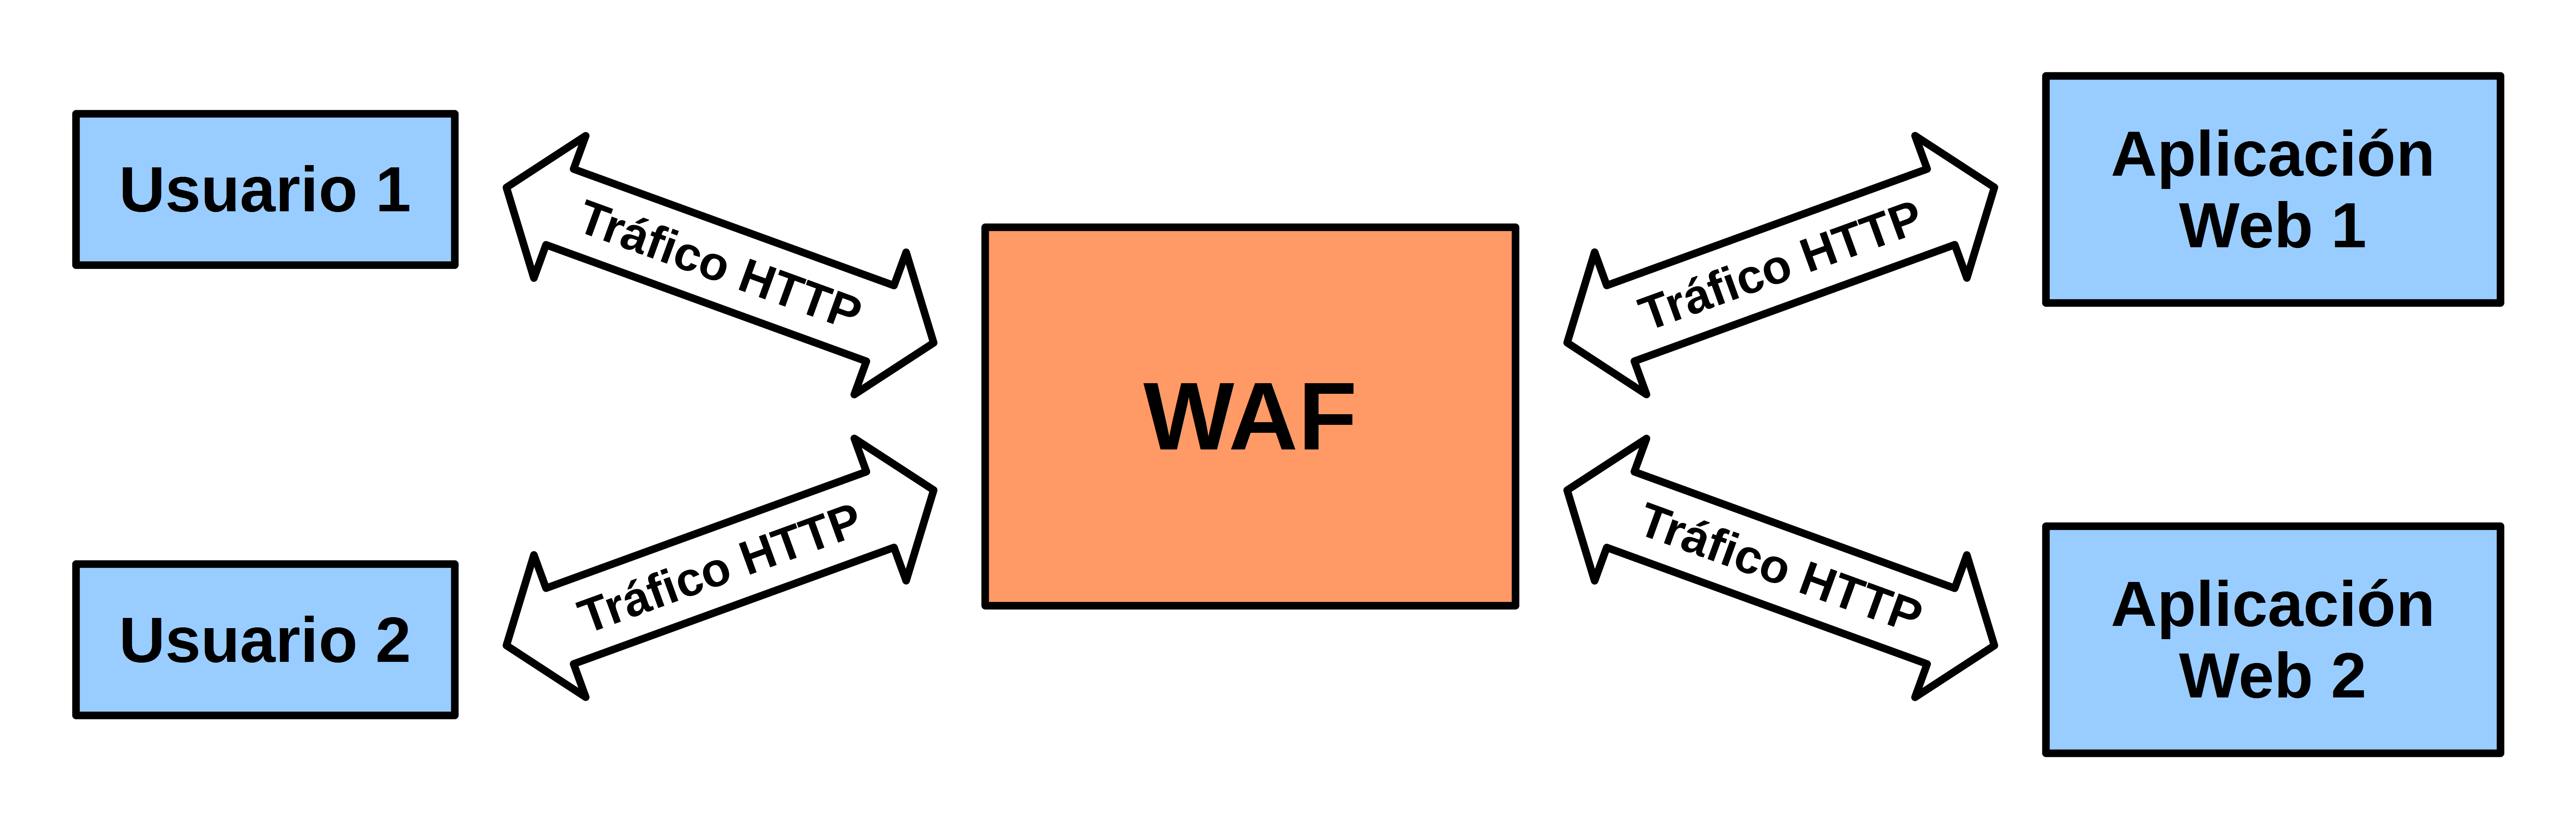
\includegraphics[width=\linewidth]{images/waf-diagram.png}
    \caption{Diagrama de la arquitectura general de la propuesta}
    \label{fig:arquitectura}
\end{figure}

La implementación tendrá la opción de habilitar o deshabilitar la detección
en tiempo real. Con la detección deshabilitada, el \gls{acr3:waf} se
limitará a registrar el tráfico para que posteriormente se pueda realizar
el entrenamiento del clasificador con muestras normales de tráfico.
Una vez entrenado, se podrá habilitar el modo de detección. En este modo
el \gls{acr3:waf} analizará todas las peticiones entrantes y registrará
todas aquellas que sean clasificadas como anómalas.
Se podrá configurar acciones adicionales que el \gls{acr3:waf} deberá
realizar como respuesta a una anomalía detectada, siendo una opción
el bloqueo de la petición en cuestión para evitar que posibles ataques
lleguen hasta las aplicaciones.


\section{Alcance y limitaciones}

Según nuestro relevamiento inicial, el trabajo de Kruegel
\cite{kruegel2003anomaly} es la investigación pionera relacionada con
\gls{acr3:ids} que se enfoca en las particularidades del tráfico HTTP,
especialmente el ánalisis de los parámetros y valores dentro de la
petición. Con más de 600 citas hasta la fecha según Google Scholar,
este trabajo ha sido utilizado como base para muchas investigaciones
posteriores.

De esta manera, la investigación del estado del arte que haremos en el
marco de nuestro trabajo se limitará a las publicaciones que citan a Kruegel
en sus referencias.
\bigskip

Para la evaluación cuantitativa de nuestro \gls{acr3:waf} propuesto
necesitamos conjuntos de datos. Según \cite{torranoGimenez2015study}
los conjuntos utilizados en las investigaciones sobre \gls{acr3:waf}
deberían cumplir las siguientes características:

\begin{itemize}
    \item
    Deberían ser públicamente accesibles para que varios investigadores
    los utilizen y puedan comparar resultados.

    \item
    Deberían contener tráfico \gls{acr3:http}.

    \item
    Deberían contener muestras etiquetadas según sean normales o
    anómalas, o inclusive especificar el tipo de ataque al que
    pertenecen.

    \item
    Deberían tener ataques novedosos.
\end{itemize}

Los trabajos relacionados sobre \gls{acr3:waf} utilizan distintos
conjuntos de datos para sus pruebas, pero la mayoria de esos
conjuntos no cumple una o varias de las características mencionadas.
Encontramos unicamente dos conjuntos que son adecuados para
nuestras pruebas y se trata de CSIC 2010 \cite{csic2010dataset} y
CSIC TORPEDA 2012 \cite{torpeda2012dataset}. Así podemos realizar
comparaciones con los resultados de otros trabajos que utilizan estos
conjuntos.
\bigskip

La implementación de un \gls{acr3:waf} que haremos en el marco de este
trabajo busca ser funcional y sencilla. Se trata de una prueba de concepto,
y no buscamos obtener una aplicación terminada que incluya todas las
funcionalidades necesarias para utilizarla directamente en ambientes de
producción.


\section{Plan de actividades}

A continuación se detallan las actividades que nosotros nos proponemos
para el desarrollo de este trabajo de investigación. Además, en la
\autoref{tbl:actividades} se puede observar las duraciones estimadas
para dichas actividades.

\begin{enumerate}
    \item
    Exploración bibliográfica sobre las áreas de \gls{acr3:ids},
    \gls{acr3:waf} y \gls{acr3:occ}, profundizando especialmente
    en trabajos que utilizan el clasificador \gls{acr3:ocsvm} y
    aquellos que basan sus \textit{features} en los trabajos de Kruegel.

    \item
    Diseño de nuevos conjuntos de \textit{features} específicos para
    tráfico \gls{acr3:http}, combinando las ideas de Kruegel con aportes
    propios y también de otros investigadores.

    \item
    Construcción de un \gls{acr3:waf} con los \textit{features} diseñados
    y con un clasificador \gls{acr3:ocsvm}.

    \item
    Pruebas de eficacia de detección del \gls{acr3:waf} construido,
    buscando conjuntos de \textit{features} y configuraciones del
    clasificador que mejoren la detección.

    \item
    Pruebas de rendimiento del \gls{acr3:waf} construido, analizando
    en qué medida el mismo afecta al tiempo de respuesta de los
    sistemas que debe proteger.

    \item
    Análisis de resultados y formulación de conclusiones.
\end{enumerate}

\begin{table}[ht]
    \centering
    \small
    \begin{tabular*}{\linewidth}{@{\extracolsep{\fill}}|l|c|c|c|c|c|c|c|c|c|c|c|c|c|c|c|c|c|c|}
        \hline
        Año & \multicolumn{18}{c|}{2017} \\ \hline
        Mes & \multicolumn{5}{c|}{Agosto} & \multicolumn{4}{c|}{Setiembre} & \multicolumn{4}{c|}{Octubre} & \multicolumn{5}{c|}{Noviembre} \\ \hline
        Semana & 1 & 2 & 3 & 4 & 5 & 1 & 2 & 3 & 4 & 1 & 2 & 3 & 4 & 1 & 2 & 3 & 4 & 5 \\ \hline \hline
        Actividad 1 & x & x & x & x & x & x & x &  &  &  &  &  &  &  &  &  &  &  \\ \hline
        Actividad 2 &  &  &  &  & x & x & x &  &  &  &  &  &  &  &  &  &  &  \\ \hline
        Actividad 3 &  &  &  &  &  &  &  & x & x & x & x &  &  &  &  &  &  &  \\ \hline
        Actividad 4 &  &  &  &  &  &  &  &  &  &  &  & x & x & x &  &  &  &  \\ \hline
        Actividad 5 &  &  &  &  &  &  &  &  &  &  &  & x & x & x &  &  &  &  \\ \hline
        Actividad 6 &  &  &  &  &  &  &  &  &  &  &  &  &  &  & x & x & x & x \\ \hline
    \end{tabular*}
    \caption{Duración estimada de actividades}
    \label{tbl:actividades}
\end{table}


    \bibliography{p5_references}
    \bibliographystyle{IEEEtran}
\end{document}
